\begin{figure*}[hbtp]
  \centering
  \subfigure[Naive-dynamic (ND) approach]{
    \label{fig:about-cases--naive}
    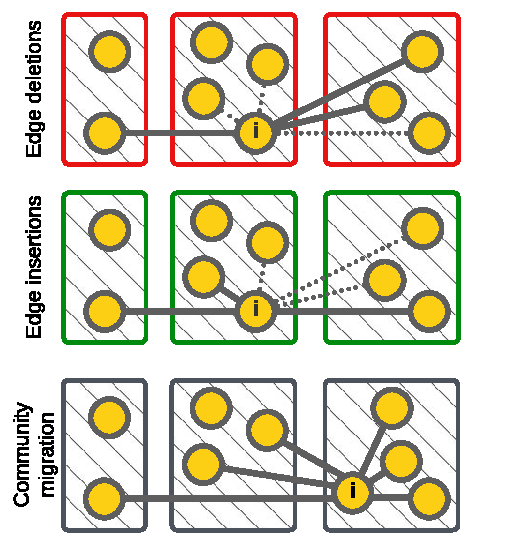
\includegraphics[width=0.3\linewidth]{out/about-cases-naive.pdf}
  }
  \subfigure[Delta-screening (DS) approach]{
    \label{fig:about-cases--delta}
    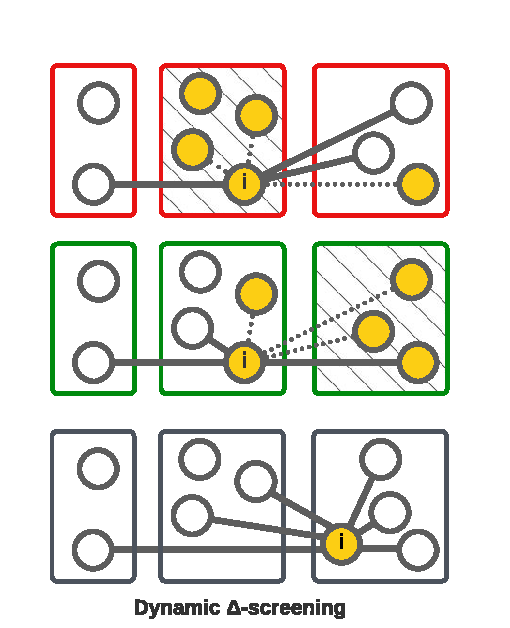
\includegraphics[width=0.3\linewidth]{out/about-cases-delta.pdf}
  }
  \subfigure[Dynamic Frontier (DF) approach]{
    \label{fig:about-cases--frontier}
    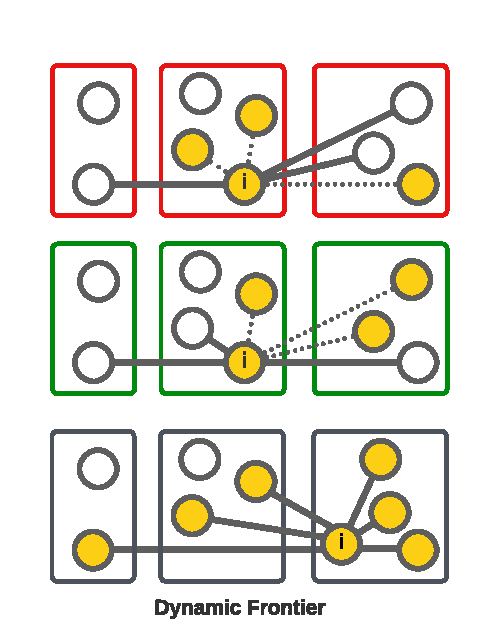
\includegraphics[width=0.3\linewidth]{out/about-cases-frontier.pdf}
  } \\[-2ex]
  \caption{Comparison of dynamic community detection approaches: \textit{Naive-dynamic (ND)}, \textit{Delta-screening (DS)}, and our \textit{Dynamic Frontier (DF)} approach. Edge deletions/insertions are indicated with dotted lines. Vertices marked as affected (initially) with each approach are highlighted in yellow, and when entire communities are marked as affected, they are hatched.}
  \label{fig:about-cases}
\end{figure*}
